Several Monte Carlo (MC) event generators are used to simulate the signal and
background processes. For all processes, the detector response is simulated using a detailed description of the CMS detector, based on the \textsc{GEANT4} 
package~\cite{Agostinelli:2002hh}, and event reconstruction is performed with
the same algorithms as used for data. Proton-proton interactions occuring in the same beam crossing bin as the event of interest (pileup) are included in the simulation samples. The simulated events are weighted so that the pileup distribution matches the data, with an average pileup of about $27$ interactions per beam crossing.

\subsection{Data samples}

This analysis uses a sample of pp collisions collected in 2016 with the CMS experiment at the LHC at $\sqrt{s} = 13~\rm{TeV}$.
Only data that passed the quality certification by all detector subsystems is used in the analysis using the golden JSON in order to select good data:
\\
\centerline{\small Cert\_271036-284044\_13TeV\_23Sep2016ReReco\_Collisions16\_JSON.txt}
\\
corresponding to an integrated luminosity of $35.9 \pm 0.9\fbinv$. {\it SingleMuon}  and {\it SingleElectron} primary datasets are used. The names of data samples used in the analysis are listed in Table~\ref{tab:datasample} 

\begin{table}[htbp]
  \caption{List of data samples used in the analysis.\label{tab:datasample}}
  \begin{center}
%{\tiny
  \begin{tabular}{l l}
\hline \textbf{Data stream} &  \textbf{Run and reconstruction version}  \\
\hline
SingleMuon      &       Run2016B-03Feb2017-v2   \\
SingleElectron  &       Run2016C-03Feb2017           \\
                &       Run2016D-03Feb2017           \\
		&       Run2016E-03Feb2017   \\
                &       Run2016F-03Feb2017           \\
		&       Run2016G-03Feb2017\\
                &       Run2016H-03Feb2017-v1  \\
		&       Run2016H-03Feb2017-v2 \\
                &       Run2016H-03Feb2017-v3\\
\hline
  \end{tabular}
%}
  \end{center}
\end{table}
 
 
\subsection{Simulated Samples}
The EW signal processes with two final state quarks are simulated using \newline \MADGRAPH{}5\_a\MCATNLO~2.3.3~\cite{Alwall:2014} at leading-order (LO) with six EW and zero quantum chromodynamics (QCD) vertices. $\PW^{\pm}\PW^{\pm}$, $\PW^{\pm}\PW^{\mp}$,$\PW^{\pm}\PZ$, and $\PZ\PZ$ processes are produced separately. The complete list of signal samples can be found in Table~\ref{tab:signalSamples}.

The QCD initiated production of two gauge bosons with two final state quarks (which we refer to as diboson process) and at least one QCD vertex is considered as background. \MADGRAPH{}5\_a\MCATNLO at LO is used to simulate this sample. The interference between the EW and QCD diagrams is evaluated using dedicated samples produced with the \textsc{Phantom}~1.2.8~\cite{Ballestrero:2007xq} generator and is found to be negligible compared to the theoretical uncertainties. Figure~\ref{fig:interference} shows the level of the interference contribution. 

\begin{figure*}[htb]
\centering
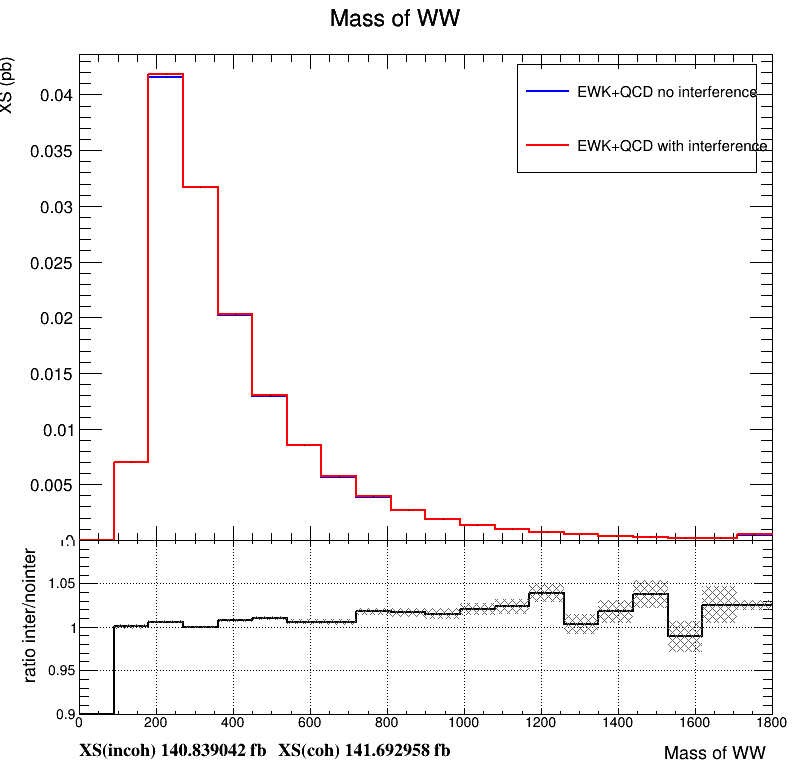
\includegraphics[width=0.9\textwidth]{Plots/plots/interference_comparison_mww.png}
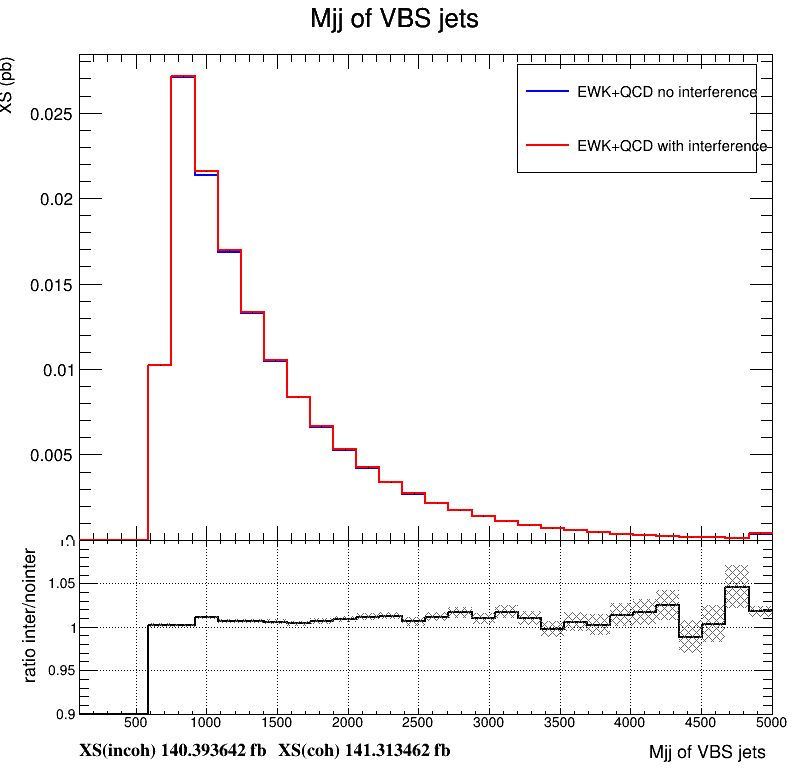
\includegraphics[width=0.9\textwidth]{Plots/plots/interference_comparison_mjj_vbs.png}
\caption{Distributions of $m_{\PW V}$ (left) and $m_{jj}$ (right) in the signal region with including the interference contribution (red) and without the intereference contribution (blue).}
\label{fig:interference}
\end{figure*}

The AQGC samples are produced using \MADGRAPH{}5\_a\MCATNLO at LO accuracy. The default coupling for the event generation is set to $f_{T0} / /Lambda^{4} = -12.5 [\mathrm{TeV}]^{-4}$. Other coupling strengths are obtained by means of the reweighing method in \MADGRAPH{}5\_a\MCATNLO. Figure~\ref{fig:aqgc_signal} shows the mass distributions of the  $\PW \PW$ system for few AQGC parameters for the operators $S0$ (left) and $T2$ (right). The expected enhancement of the production cross section at large masses for nonzero AQGC is clearly seen.      
  
\begin{figure*}[htb]
\centering
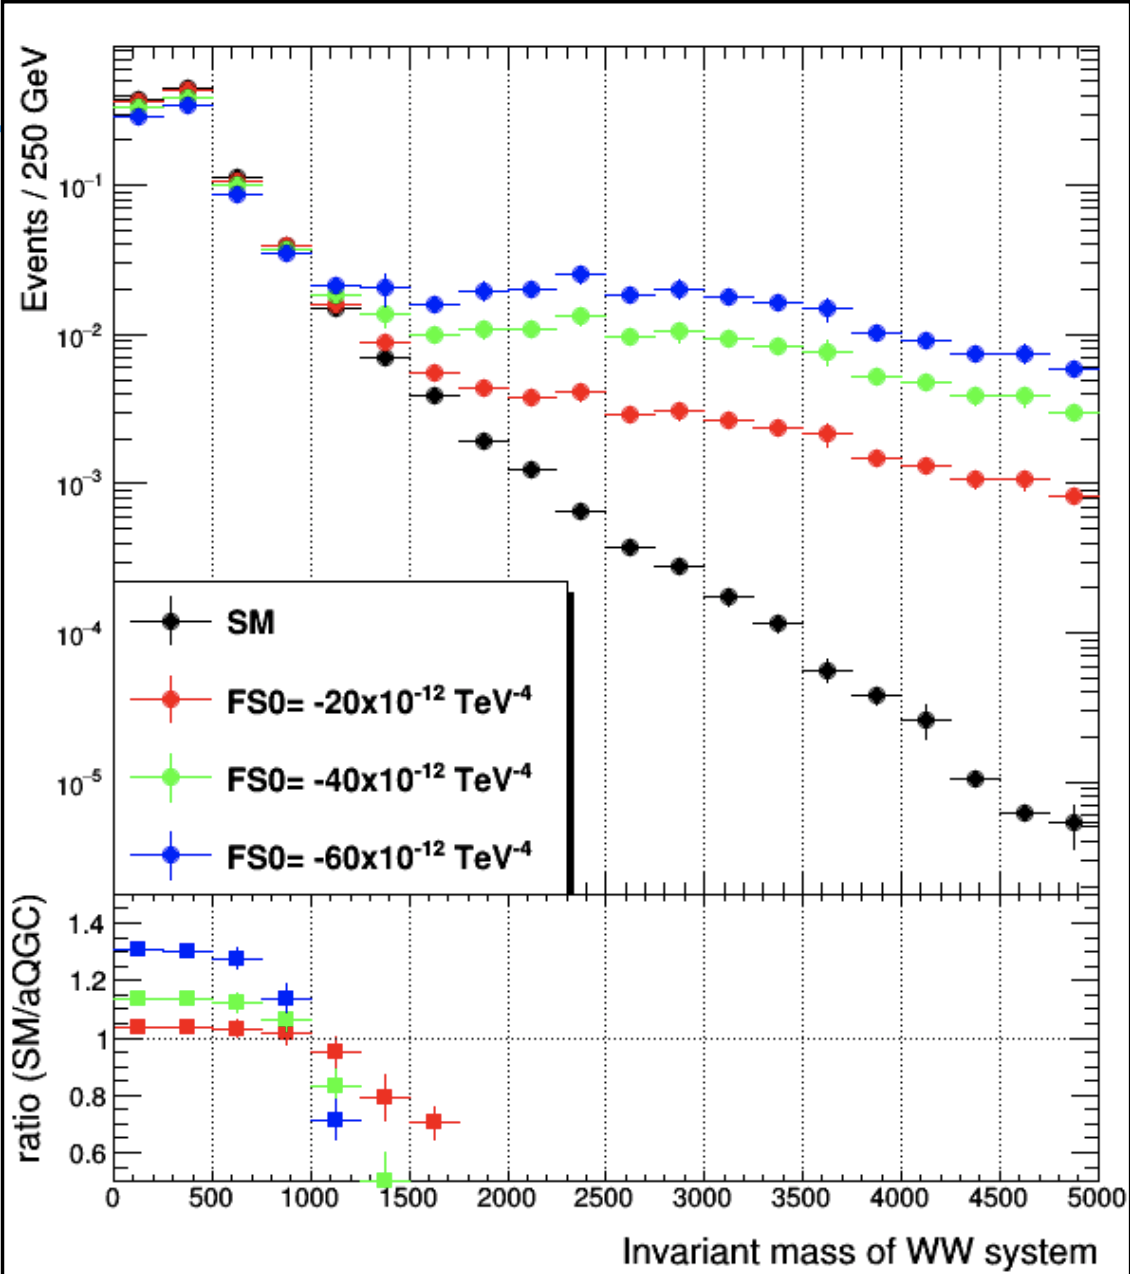
\includegraphics[width=0.9\textwidth]{Plots/aQGC_Signal_Scaling/mWW_FS0.png}
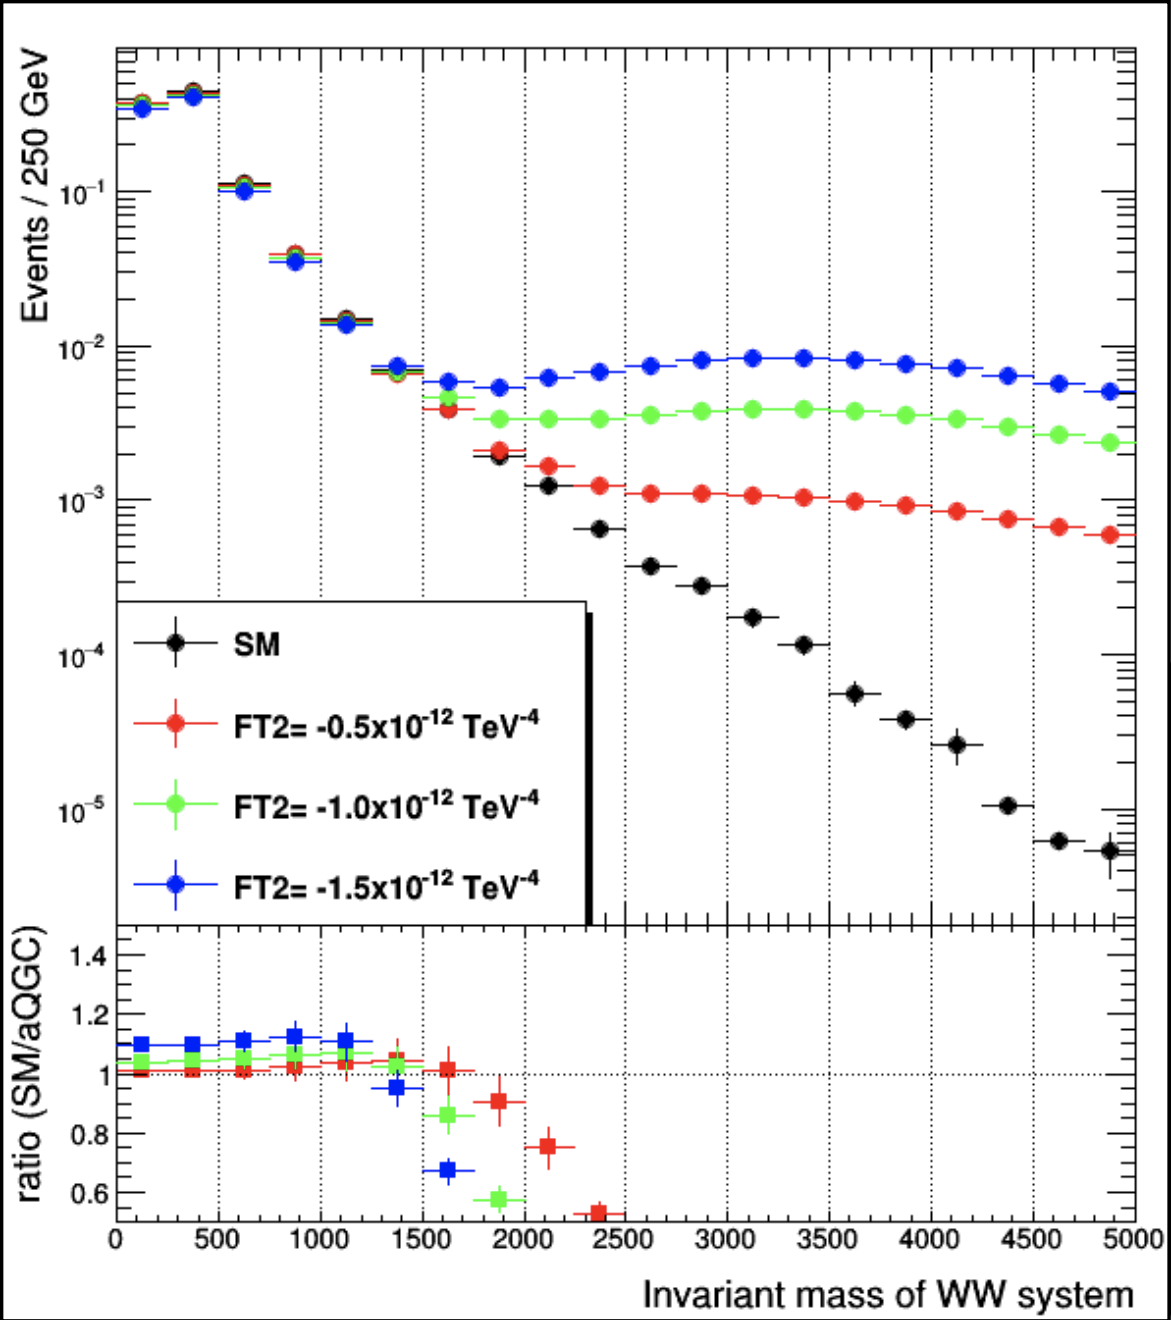
\includegraphics[width=0.9\textwidth]{Plots/aQGC_Signal_Scaling/mWW_FT2.png}
\caption{Mass distributions of the $\PW \PW$ system for the SM EW and few AQGC parameters for the operators $S0$ (left) and $T2$ (right).}
\label{fig:aqgc_signal}
\end{figure*}


\begin{table}[htbp]
\footnotesize
\centering
\topcaption{Signal sample names and cross sections of simulated samples used in the analysis}
\begin{tabular}{lrr}
\textbf{Sample name} & \textbf{Total events} & \textbf{Cross section[pb]} \\
\hline
/WplusToLNuWminusTo2JJJ\tus{}EWK\tus{}LO\tus{}SM\tus{}*	&	1,991,279	&	0.9114\\
/WplusTo2JWminusToLNuJJ\tus{}EWK\tus{}LO\tus{}SM\tus{}*	&	1,994,040	&	0.9107\\
/WplusToLNuWplusTo2JJJ\tus{}EWK\tus{}LO\tus{}SM\tus{}*	&	198,858		&	0.0879\\
/WminusToLNuWminusTo2JJJ\tus{}EWK\tus{}LO\tus{}SM\tus{}*	&	199,535		&	0.0326\\
/WplusToLNuZTo2JJJ\tus{}EWK\tus{}LO\tus{}SM\tus{}*		&	393,190		&	0.1825\\
/WplusTo2JZTo2LJJ\tus{}EWK\tus{}LO\tus{}SM\tus{}*			&	198,932		&	0.0540\\
/WminusToLNuZTo2JJJ\tus{}EWK\tus{}LO\tus{}SM\tus{}*		&	199,547		&	0.1000\\
/WminusTo2JZTo2LJJ\tus{}EWK\tus{}LO\tus{}SM\tus{}*		&	198,910		&	0.0298\\
/ZTo2LZTo2JJJ\tus{}EWK\tus{}LO\tus{}SM\tus{}*				&	100,000		&	0.0159\\
\hline
\hline
/WplusToLNuWminusTo2JJJ\tus{}EWK\tus{}LO\tus{}aQGC\tus{}*	&	1,981,940	&	17.940\\
/WplusTo2JWminusToLNuJJ\tus{}EWK\tus{}LO\tus{}aQGC\tus{}*	&	1,994,595	&	17.920\\
/WplusToLNuWplusTo2JJJ\tus{}EWK\tus{}LO\tus{}aQGC\tus{}*	&	200,000		&	3.451\\
/WminusToLNuWminusTo2JJJ\tus{}EWK\tus{}LO\tus{}aQGC\tus{}*&	200,000		&	0.507\\
/WplusToLNuZTo2JJJ\tus{}EWK\tus{}LO\tus{}aQGC\tus{}*		&	399,232		&	1.895\\
/WplusTo2JZTo2LJJ\tus{}EWK\tus{}LO\tus{}aQGC\tus{}*		&	199,238		&	0.569\\
/WminusToLNuZTo2JJJ\tus{}EWK\tus{}LO\tus{}aQGC\tus{}*		&	200,000		&	0.741\\
/WminusTo2JZTo2LJJ\tus{}EWK\tus{}LO\tus{}aQGC\tus{}*		&	198,620		&	0.222\\
/ZTo2LZTo2JJJ\tus{}EWK\tus{}LO\tus{}aQGC\tus{}*			&	99,532		&	3.361\\
\hline
* = MJJ100PTJ10\tus{}TuneCUETP8M1\tus{}13TeV-madgraph-pythia8/ \\
    RunIISummer16MiniAODv2-PUMoriond17\tus{}80X\tus{}mcRun2\tus{}\\
    asymptotic\tus{}2016\tus{}TrancheIV\tus{}v6-v1/MINIAODSIM\\
\hline
\end{tabular}
\label{tab:signalSamples}
\end{table}

The Drell--Yan process is simulated with one, two, three, and four outgoing partons at Born level at LO using \MADGRAPH{}5\_a\MCATNLO. $\PW+$jet process is simulated at LO in $\mathrm{H_{T}}$ bins using \MADGRAPH{}5\_a\MCATNLO. $\ttbar$, $\ttbar \PW$, $\ttbar \PZ$, and single top processes are generated at nest-to-leading order (NLO) using \textsc{POWHEG2.0}~\cite{Alioli:2008gx,Nason:2004rx,Frixione:2007vw,powheg:2010}. The simulated samples of background processes are normalized to the best theoretical prediction. The complete list of background samples can be found in Table~\ref{tab:bkgSamples}.

The \PYTHIA~8.205~\cite{Sjostrand:2015} package is used  for parton showering, hadronization, and the underlying event simulation, with tune CUETP8M1~\cite{Skands:2014pea,Khachatryan:2015pea}. The NNPDF~3.0~\cite{nnpdf} set is used as the default set of parton distribution functions (PDFs). The PDFs are calculated to the same order in QCD as the hard process. 

\begin{table}[htbp]
\footnotesize
\centering
\topcaption{Sample names and cross sections of simulated samples used in the analysis.}
\begin{tabular}{lrr}
\textbf{Sample name} & \textbf{Cross section[pb]} \\
\hline
WJetsToLNu\tus{}HT-100To200\tus{}TuneCUETP8M1\tus{}13TeV-madgraphMLM-pythia8  & 1345*1.21 \\
WJetsToLNu\tus{}HT-200To400\tus{}TuneCUETP8M1\tus{}13TeV-madgraphMLM-pythia8 & 359.7*1.21 \\
WJetsToLNu\tus{}HT-400To600\tus{}TuneCUETP8M1\tus{}13TeV-madgraphMLM-pythia8 & 48.91*1.21 \\
WJetsToLNu\tus{}HT-600To800\tus{}TuneCUETP8M1\tus{}13TeV-madgraphMLM-pythia8 & 12.05*1.21 \\
WJetsToLNu\tus{}HT-800To1200\tus{}TuneCUETP8M1\tus{}13TeV-madgraphMLM-pythia8 & 5.501*1.21 \\
WJetsToLNu\tus{}HT-1200To2500\tus{}TuneCUETP8M1\tus{}13TeV-madgraphMLM-pythia8 & 1.329*1.21 \\
WJetsToLNu\tus{}HT-2500ToInf\tus{}TuneCUETP8M1\tus{}13TeV-madgraphMLM-pythia8 & 0.03216*1.21 \\
\hline
WplusToLNuWminusTo2JJJ\tus{}EWK\tus{}LO\tus{}QCD\tus{}*	&	5.544\\
WplusTo2JWminusToLNuJJ\tus{}EWK\tus{}LO\tus{}QCD\tus{}*	&	5.561\\
WplusToLNuWplusTo2JJJ\tus{}EWK\tus{}LO\tus{}QCD\tus{}*	        &	0.08642\\
WminusToLNuWminusTo2JJJ\tus{}EWK\tus{}LO\tus{}QCD\tus{}*       &	0.03774\\
WplusToLNuZTo2JJJ\tus{}EWK\tus{}LO\tus{}QCD\tus{}*		&	2.162\\
WplusTo2JZTo2LJJ\tus{}EWK\tus{}LO\tus{}QCD\tus{}*		&	0.6409\\
WminusToLNuZTo2JJJ\tus{}EWK\tus{}LO\tus{}QCD\tus{}*		&	1.302\\
WminusTo2JZTo2LJJ\tus{}EWK\tus{}LO\tus{}QCD\tus{}*		&	0.3862\\
ZTo2LZTo2JJJ\tus{}EWK\tus{}LO\tus{}QCD\tus{}*			&	0.3756\\
\hline
TT\tus{}TuneCUETP8M1\tus{}13TeV-powheg-pythia8 & 831.76 \\
\hline
ST\tus{}s-channel\tus{}4f\tus{}leptonDecays\tus{}13TeV-amcatnlo-pythia8\tus{}TuneCUETP8M1 & 3.68 \\
ST\tus{}t-channel\tus{}top\tus{}4f\tus{}inclusiveDecays\tus{}13TeV-powhegV2-madspin-pythia8\tus{}TuneCUETP8M1 & 136.02 \\
ST\tus{}t-channel\tus{}antitop\tus{}4f\tus{}inclusiveDecays\tus{}13TeV-powhegV2-madspin-pythia8\tus{}TuneCUETP8M1 & 80.95 \\
ST\tus{}tW\tus{}antitop\tus{}5f\tus{}inclusiveDecays\tus{}13TeV-powheg-pythia8\tus{}TuneCUETP8M1 & 35.6 \\
ST\tus{}tW\tus{}top\tus{}5f\tus{}inclusiveDecays\tus{}13TeV-powheg-pythia8\tus{}TuneCUETP8M1 & 35.6 \\
\hline
DY1JetsToLL\_M-50\_TuneCUETP8M1\_13TeV-madgraphMLM-pythia8 & 1012 \\
DY2JetsToLL\_M-50\_TuneCUETP8M1\_13TeV-madgraphMLM-pythia8 & 335 \\
DY3JetsToLL\_M-50\_TuneCUETP8M1\_13TeV-madgraphMLM-pythia8 & 102 \\
DY4JetsToLL\_M-50\_TuneCUETP8M1\_13TeV-madgraphMLM-pythia8 & 54 \\
%QCD\_HT200to300\_TuneCUETP8M1\_13TeV-madgraphMLM-pythia8 & 1717000 \\
%QCD\_HT300to500\_TuneCUETP8M1\_13TeV-madgraphMLM-pythia8 & 351300 \\
%QCD\_HT500to700\_TuneCUETP8M1\_13TeV-madgraphMLM-pythia8 & 31630 \\
%QCD\_HT700to1000\_TuneCUETP8M1\_13TeV-madgraphMLM-pythia8 & 6802 \\
%QCD\_HT1000to1500\_TuneCUETP8M1\_13TeV-madgraphMLM-pythia8 & 1206 \\
%QCD\_HT1500to2000\_TuneCUETP8M1\_13TeV-madgraphMLM-pythia8 & 120.4 \\
%QCD\_HT2000toInf\_TuneCUETP8M1\_13TeV-madgraphMLM-pythia8 & 25.25 \\
%\hline
\end{tabular}
\label{tab:bkgSamples}
\end{table}
